A partir de los datos de los casos penales, pudimos
para construir la red de Grupos de Pertenencia. En esta red, ............. Una visualización de la red se representa en la
Figura 1 y hemos incluido estadísticas de resumen en la Tabla 2.
Al estudiar esta red, estudiamos su distribución.......................
(Figura 2). 

\begin{figure}
	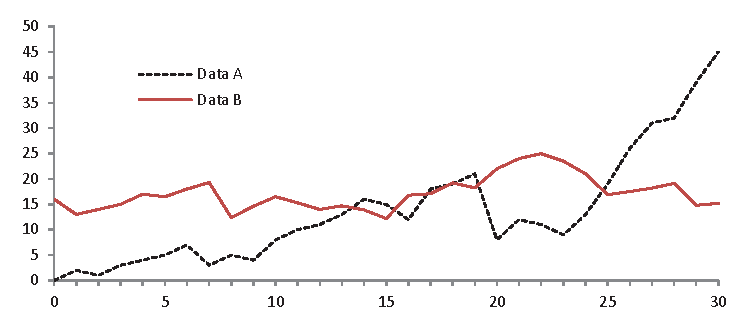
\includegraphics[width=\textwidth]{fig1.eps}
	\caption{Descripción de la figura1.} \label{fig1}
\end{figure}

\begin{table}
	\caption{Descripción de la tabla2}\label{tab2}
\end{table}

\begin{figure}
	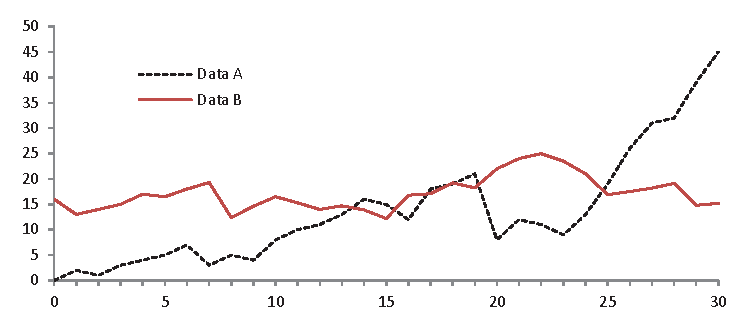
\includegraphics[width=\textwidth]{fig1.eps}
	\caption{Descripción de la figura2.} \label{fig2}
\end{figure}